\section{考察}

\subsection{実験装置の改良に伴う擬塑性流体への落下への影響}

今回,球を把持する手法を,電磁石を用いて把持する方法から真空ポンプを用いて把持する方法に変化させた.すると,落下開始時0-0.3sにおける,落下速度のオーバーシュートが,先行研究より小さくなった.この落下速度のオーバーシュートは弾性による影響によって生じることが示されている\cite{ref:12}.以下で,オーバーシュートが顕著に見られなかった原因を,物質の流動性を表す$De$数より考える.$De$数が大きくなると,弾性的傾向が強くなり,$De$数が小さくなると,粘性的流動を表す.

$De$数は下記の様に緩和時間$\lambda$[s],代表時間$T$[s]の比で表される.
\begin{equation}
    De = \frac{\lambda}{T} .
    \label{eq:De}
\end{equation}
代表時間$T$[s]に関して,超音波照射を行っていない場合の球の落下条件においても考えるため,
\begin{equation}
    T = \frac{a}{U} ,
    \label{eq:T}
\end{equation}
となる.ここで,球の落下速度$U$[m/s],球の半径$a$[m]である.また,緩和時間$\lambda$[s]は,
\begin{equation}
    \lambda \approx \frac{\mu}{G'} .
    \label{eq:lamda}
\end{equation}
ここで粘度$\mu$[Pa$\times$s],貯蔵弾性率$G'$[Pa]である.緩和時間は変形の経過時間において,粘弾性流体が流体的挙動を示すか,固体的挙動を示すかの指標である\cite{ref:sakanishi}.粘度$\mu$[Pa$\times$s]に関して,せん断速度$\dot{\gamma}$[1/s]および粘度定数$k$[Pa$\times$s${}^n$],指数$n$を用いてPower-law modelに従うとすると,
\begin{equation}
    \mu = k \times \dot{\gamma}^{n-1} ,
    \label{eq:power-law}
\end{equation}
となる.せん断速度$\dot{\gamma}$[1/s]に関して,球の落下による影響を考えるため,
\begin{equation}
    \dot{\gamma} \sim \frac{U}{a} ,
    \label{eq:gamma}
\end{equation}
となる.よって,式\ref{eq:power-law},\ref{eq:gamma}より粘度$\mu$は
\begin{equation}
    \mu \sim k \times \left(\frac{U}{a}\right)^{n-1} ,
    \label{eq:power-law2}
\end{equation}
と表される.これら式\ref{eq:De},\ref{eq:T},\ref{eq:lamda},\ref{eq:power-law2}より,$De$数は,
\begin{equation}
    De \sim \frac{k}{G'} {\left(\frac{U}{a}\right)}^n ,
    \label{eq:De2}
\end{equation}
となり,粘度定数$k$[Pa$\times$s${}^n$],貯蔵弾性率$G'$[Pa],落下速度$U$[m/s],球の半径$a$[m]によって表される.

貯蔵弾性率$G'$[Pa]に関して,先行研究において計測されたFig.\ref{fig:iwamuro-G}(b)の結果より考える.この図において,貯蔵弾性率$G'$[Pa]は応力$\tau$[Pa]との関係性が示されている.ここで応力$\tau$[Pa]は,
\begin{equation}
    \tau = \mu \times \dot{\gamma} ,
    \label{eq:tau}
\end{equation}
となる.ここに,式\ref{eq:power-law},\ref{eq:gamma}を代入すると,
\begin{equation}
    \tau \sim k \times \left(\frac{U}{a}\right)^n , 
    \label{eq:tau-cal}
\end{equation}
となる.

Fig.\ref{fig:falling-A}, \ref{fig:iwamuro-fall}それぞれの結果より,ピーク速度$U_{peak}$[mm/s]と終端速度$U_{ave}$[mm/s]を算出した.続いて,式\ref{eq:tau-cal}を用いて,それぞれの速度における応力$\tau_{peak}$[Pa],$\tau_{ave}$[Pa]の算出を行った.これら算出結果と先行研究の計測結果Fig.\ref{fig:iwamuro-G}より,貯蔵弾性率$G'$も求めた.これらの結果を,Table\ref{table:iwamuro}に示す.

また,式\ref{eq:power-law2}を用いて,ピーク速度/終端速度それぞれの粘度$\mu_{peak}$[Pa$\cdot$s],$\mu_{ave}$[Pa$\cdot$s]を概算した.これらの粘度を式\ref{eq:lamda}に代入し,それぞれの緩和時間$\lambda_{peak}$[s],$\lambda_{ave}$[s]の算出を行った.そして,それらの緩和時間より,式\ref{eq:De}を用いて,それぞれの$De$数,$De_{peak}$,$De_{ave}$を求めた.これらの結果を,Table \ref{table:iwamuro2}に示す.

Table \ref{table:iwamuro2}より,ピーク速度より求めた$De_{peak}$と,終端速度より求めた$De_{ave}$において,それぞれに顕著な差異が見られないことが分かった.以降,$De_{peak}$に関してのみ議論を行う.$De_{peak}$に関して,球の半径との関係性をFig.\ref{fig:a-Degraph}に示す.横軸は半径$a$[mm],縦軸は$De$数である.先行研究であるIwamuro \textit{et al.}\cite{ref:8}の結果に関して,球の半径が大きくなると,それに伴い$De$数も増加していることが分かった.式\ref{eq:De2}において,球の半径$a$が増加すると$De$数は減少すると考えられるが,落下速度$U$のが大きく変化したためと考えられる.

一方で,真空ポンプを用いた落下実験(niwa exp.)の$De$数は,先行研究の結果において球の半径$4<a<4.5$[mm]の間における$De$数に相当すると考えられる.真空ポンプを用いた落下実験の場合,$De$数が小さくなった原因であるが,ピーク速度$U_{peak}$が小さかったためと考えられる.電磁石を用いて把持した場合,落下開始時に初速を与える必要がある.一方で,真空ポンプを用いて把持した場合,初速を与えず落下を開始することができる.このように初速の有無が影響の一つとして考えられる.これを検証するため,球を液面上部の空中から落下させ,初速を与えた状態で溶液中へ落下させる実験を行う必要があると考えられる.

\begin{table}[hbtp]
    \caption{Peak velocity $U_{peak}$/ end velocity $U_{ave}$, stress $\tau$, storage modulus $G'$ Calculation result.}
    \label{table:iwamuro}
    \centering
    \begin{tabular}{ccccccc}
      \hline
      \multirow{2}{*}{実験者} & 球直径[mm] & ピーク速度[mm/s] & 終端速度[mm/s] &\multicolumn{2}{c}{応力[Pa]} & 貯蔵弾性率[Pa] \\
       & $D=2a$ & $U_{peak}$ & $U_{ave}$ &  $\tau_{peak}$ & $\tau_{ave}$ & $G'$\\
      \hline \hline
      \multirow{8}{*}{Iwamuro} & 3  & 10.08 & 9.05 & 14.6 & 14.2 & 8\\
      & 4  & 23.2 & 19.4 & 16.5 & 15.9 & 7\\
      & 5  & 34.8 & 32.6 & 17.2 & 17.0 & 6.7 \\
      & 6  & 46.3 & 54.8 & 17.6 & 18.3 & 6.5\\
      & 7  & 79.8 & 82 & 19.3 & 19.4 & 5.5\\
      & 8  & 130 & 113 & 20.9 & 20.3 & 5 \\
      & 9  & 193 & 133 & 22.3 & 20.5 & 4\\
      & 10 & 256 & 168 & 23.2 & 21.2 & 3.5\\
      \hline \hline
      Niwa & 10 & 148 & 144 & 18.9 & 18.7 & 6 \\
      \hline
    \end{tabular}
\end{table}
\begin{table}[hbtp]
    \caption{Viscosity $\mu$, Relaxation time $\lambda$, number of $De$ Calculation result.}
    \label{table:iwamuro2}
    \centering
    \begin{tabular}{ccccccccc}
      \hline
      \multirow{2}{*}{実験者} & 球直径 &\multicolumn{2}{c}{粘度[Pa$\cdot$s]} &\multicolumn{2}{c}{緩和時間[s]}  &\multicolumn{2}{c}{$De$数[-]} \\
       & $D=2a$[mm] & $\mu_{peak}$ & $\mu_{ave}$  &  $\lambda_{peak}$ & $\lambda_{ave}$ & $De_{peak}$ & $De_{ave}$ \\
      \hline \hline
      \multirow{8}{*}{Iwamuro} & 3  & 2.17 & 2.36 & 0.27 & 0.29 & 1.82 & 1.78\\
      & 4  & 1.42 & 1.63 & 0.20 & 0.23 & 2.36 & 2.26\\
      & 5  & 1.24 & 1.30 & 0.18 & 0.19 & 2.57 & 2.53 \\
      & 6  & 1.14 & 1.00 & 0.18 & 0.15 & 2.71 & 2.82\\
      & 7  & 0.85 & 0.83 & 0.15 & 0.15 & 3.51 & 3.53\\
      & 8  & 0.64 & 0.72 & 0.13 & 0.14 & 4.19 & 4.05 \\
      & 9  & 0.52 & 0.69 & 0.13 & 0.17 & 5.58 & 5.12\\
      & 10 & 0.45 & 0.63 & 0.13 & 0.18 & 6.64 & 6.03\\
      \hline \hline
      Niwa & 10 & 0.64 & 0.65 & 0.11 & 0.11 & 3.15 & 3.12 \\
      \hline
    \end{tabular}
\end{table}
\begin{figure}[ht]
    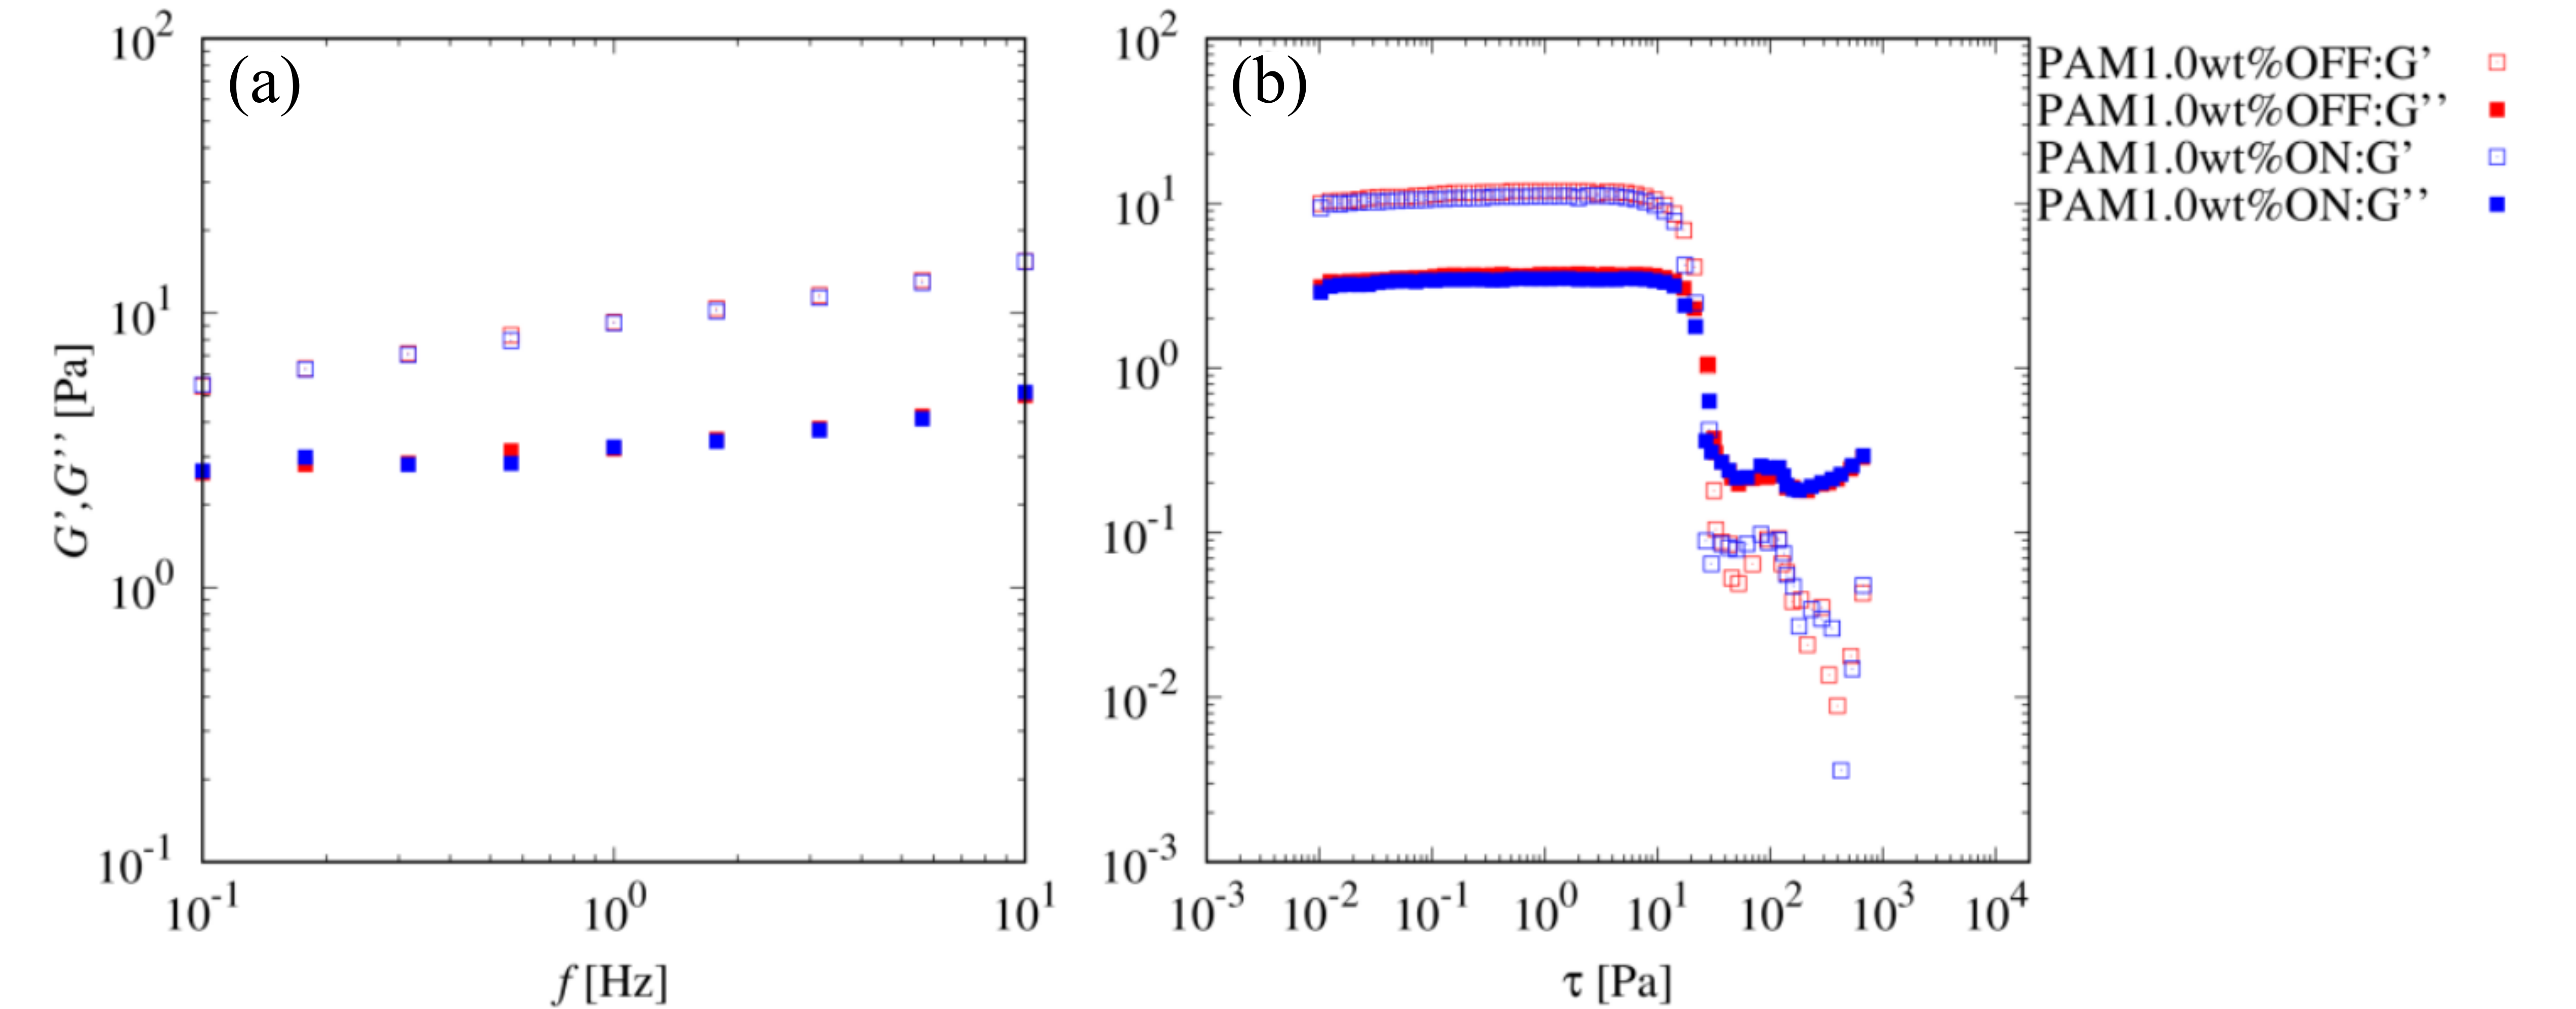
\includegraphics[width=15cm,clip]{5-Discussion/iwamuro-G.PNG}
    \caption{Frequency and stress dependence of storage and loss moduli for 1.0 wt.\% PAA.\cite{ref:8}}
    \label{fig:iwamuro-G}
\end{figure}

\begin{figure}[ht]
    \begin{center}
        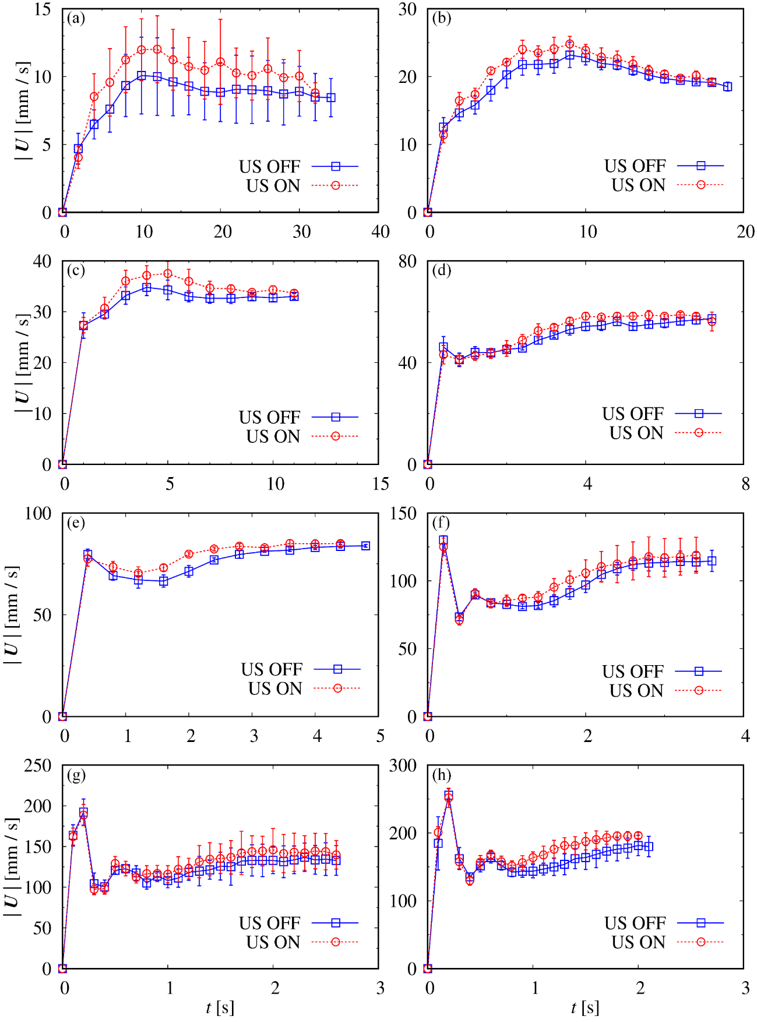
\includegraphics[width=13cm,clip]{5-Discussion/iwamuro-fall.png}
    \caption{Velocity of a falling sphere in diameter of (a) 3 mm, (b) 4 mm, (c) 5 mm, (d) 6 mm, (e) 7 mm, (f) 8 mm, (g) 9 mm, (h) 10 mm in 1.0 wt.\% PAA solution with ultrasound fixed frequency at 27.4 kHz and $\Delta \bar{P} \approx$ 180 kPa\cite{ref:8}.}
    \label{fig:iwamuro-fall}
    \end{center}
\end{figure}

\begin{figure}[ht]
    \begin{center}
        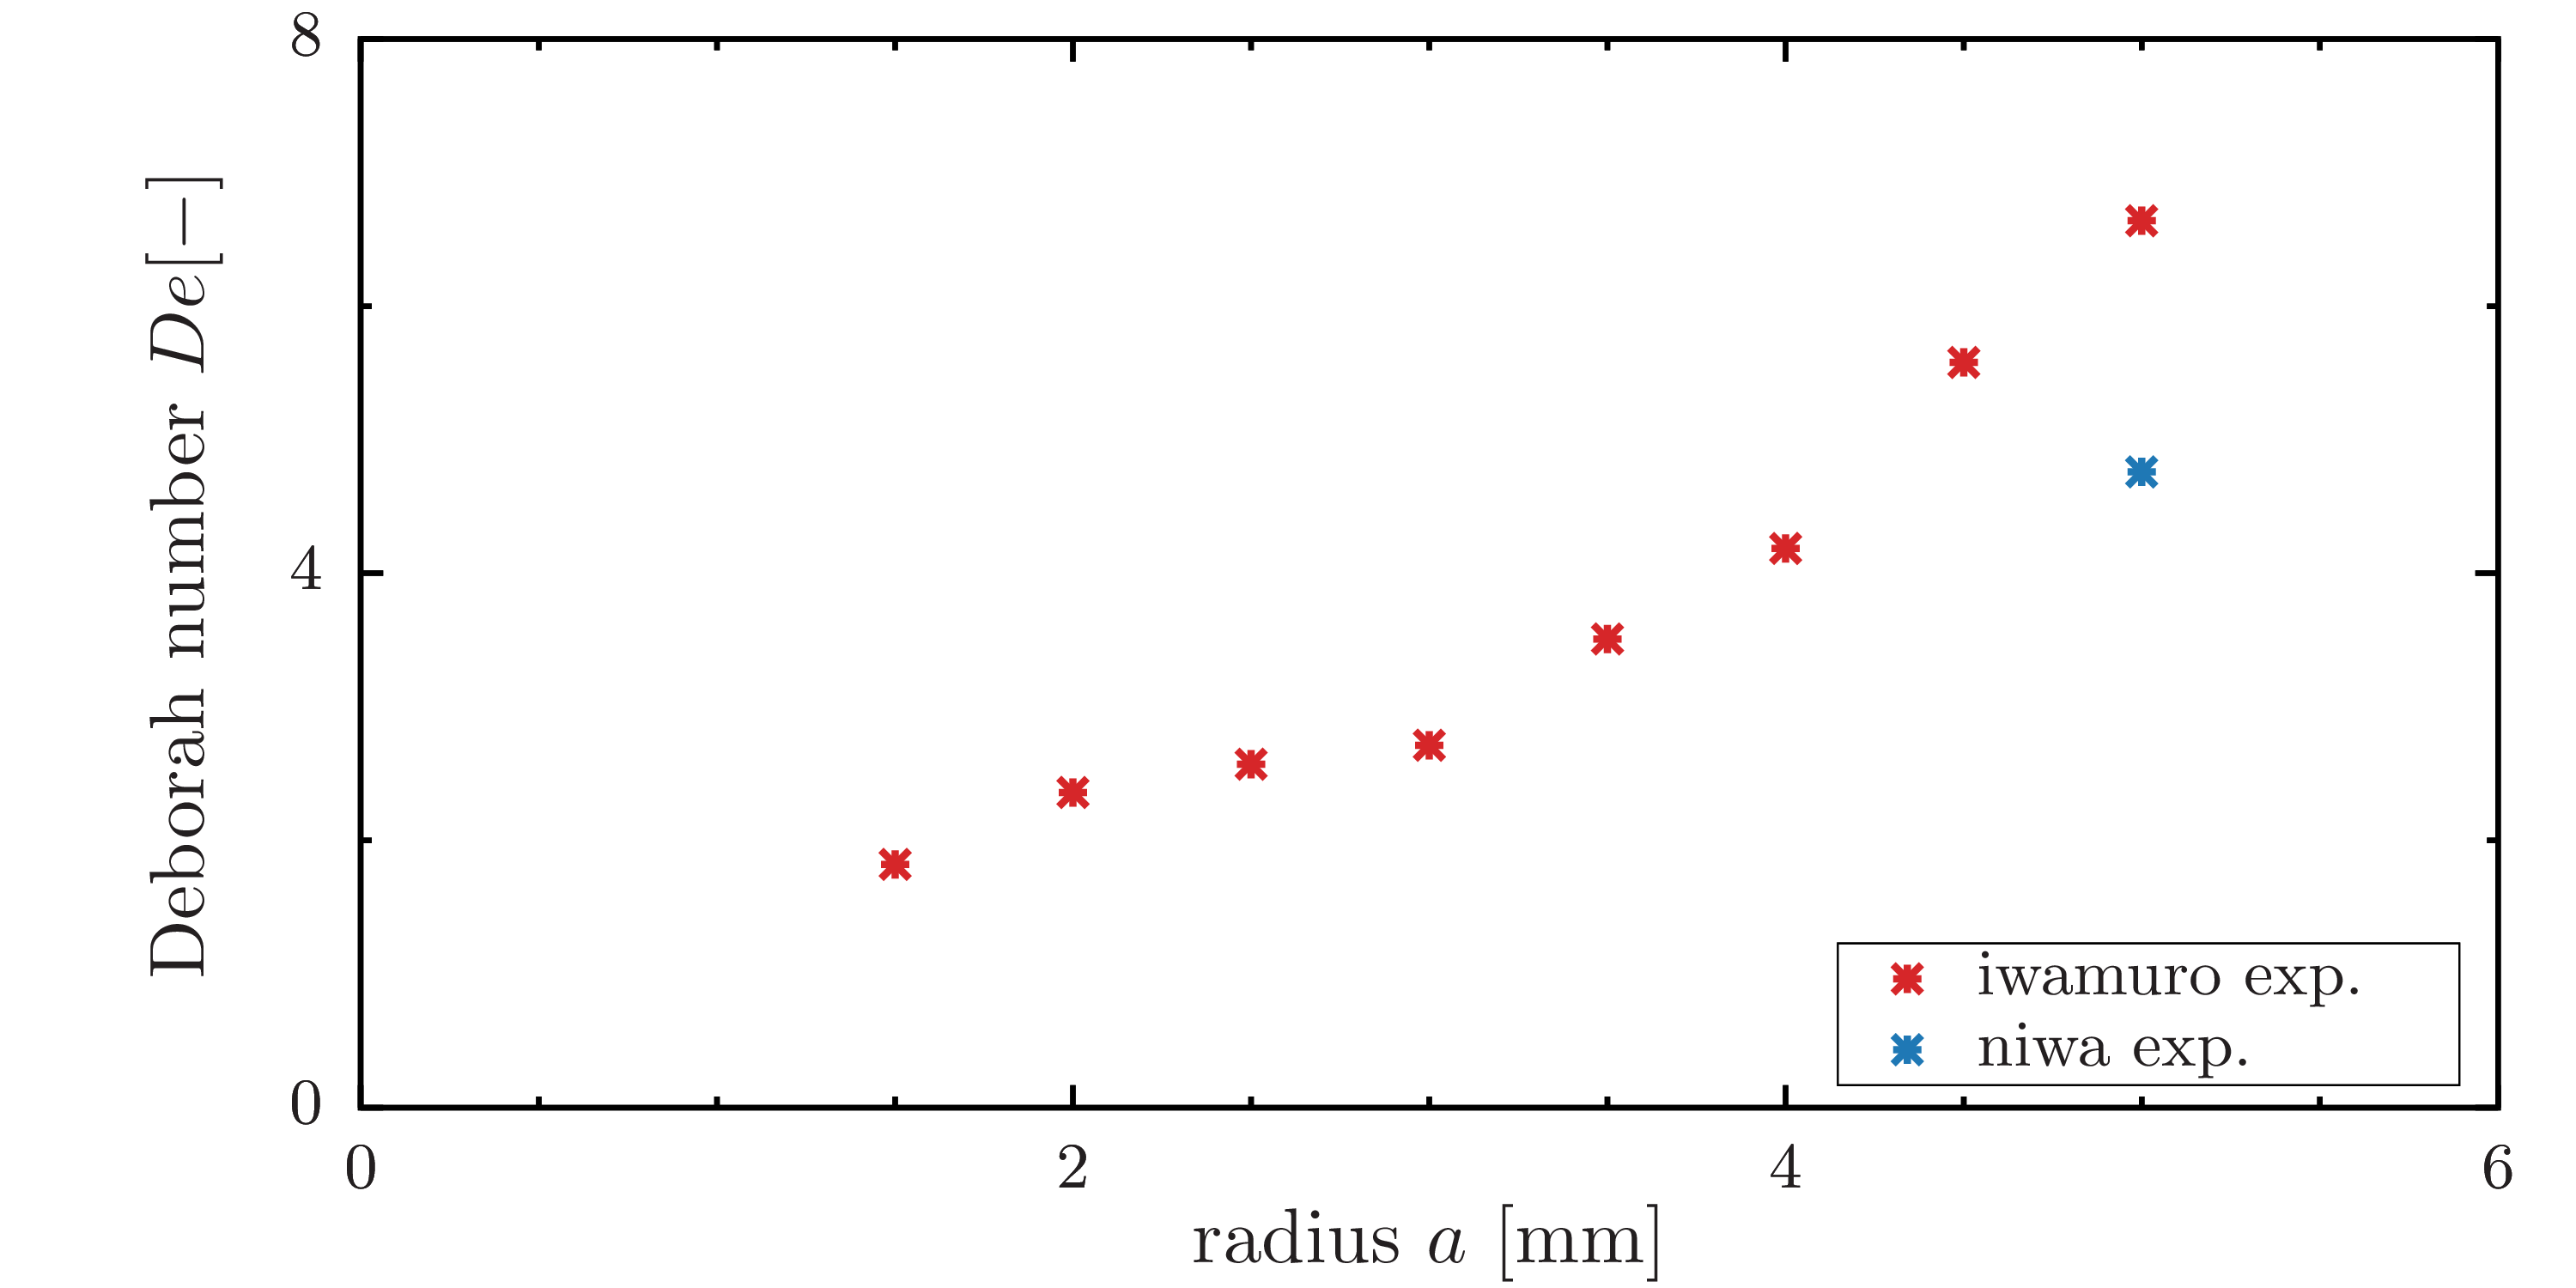
\includegraphics[width=15cm,clip]{5-Discussion/Deborah.png}
        \caption{Relationship between the radius $a$ and the number $De$ of falling spheres.}
        \label{fig:a-Degraph}
    \end{center}
\end{figure}

\clearpage

\subsection{落下間隔変化における超音波照射による高速化}

球の落下間隔を5分,10分,20分と変化させた.その結果をFig.\ref{fig:interval-change}に示す.なお,縦軸は落下速度[mm/s],横軸は落下開始時からの経過時間[s]である.全ての条件において超音波照射に伴う高速化は見られた.また落下速度は,落下間隔10分,5分,20分の順で速かった.この結果を元に,超音波照射時の球の落下速度$U_{on}$と超音波照射なしの球の落下速度$U_{off}$として,速度比$U_{on}/U_{off}$を求めた.その結果をFig.\ref{fig:speed-diff}に示す.ここで縦軸は速度比[-],横軸は落下間隔時間[min]である.この結果より,落下速度と同様に,落下間隔10分,5分,20分の順で超音波照射による高速化が見られた.このことに関して,超音波照射による高速化のメカニズムより考える.

超音波照射を行っていない状態で,擬塑性流体中を落下する球の終端速度$U_T$は下記の様に見積もられる\cite{ref:8}.
\begin{eqnarray}
    U_T \sim \frac{a^3\Delta\rho g}{3}  \int^{\infty}_{a} \frac{dr}{\mu r^2} \sim \left(\frac{\Delta \rho g}{3k}\right)^{\frac{1}{n}}\frac{n}{2-n}a^{\frac{n+1}{n}} .
    \label{eq:UT}
\end{eqnarray}
ここで,球と流体の密度差$\Delta \rho$,重力加速度$g$である.この式より,粘度が小さくなると,終端速度が大きくなることが分かる.

続いて,超音波照射に伴う高速化における粘度の影響について考える.音響境界層厚さ$\delta$は,次のように表される.
\begin{eqnarray}
    \delta \sim \left(\frac{k\left(\Delta P\right)^{n-1}}{\pi \rho^n_1 c^{n-1} f}\right)^{\frac{1}{n+1}} .
    \label{eq:delta}
\end{eqnarray}

ここで,音響圧$\Delta P$,水溶液密度$\rho_1$,音速$c$,周波数$f$である.音響境界層粘度$\mu_{ABL}$とすると超音波照射下における終端速度$U_{ABL}$は,式\ref{eq:UT}より,
\begin{eqnarray}
    U_{ABL} \sim \frac{a^3\Delta\rho g}{3}  \int^{\infty}_{a} \frac{dr}{\mu_{ABL} r^2} \sim \frac{a\Delta \rho \delta g}{3\mu_{ABL}} ,
    \label{eq:U_ABL}
\end{eqnarray}
と見積もられる.ある粘度$\mu_0$における終端速度を$U_0$とする.式\ref{eq:UT},\ref{eq:U_ABL}より,超音波照射の有無による終端速度比は,
\begin{eqnarray}
    \frac{U_{ABL}}{U_0} \sim \frac{\mu_0}{\mu_{ABL}}\frac{\delta}{a} ,
    \label{eq:Udiff}
\end{eqnarray}
と表される.また,音響境界層粘度$\mu_{ABL}$は
\begin{eqnarray}
    \mu_{ABL} \sim k\left(\frac{u}{\delta}\right)^{n-1} ,
    \label{eq:muABL}
\end{eqnarray}
と見積もられる.ここで,$u$は音波によって加振される流体粒子速度を表す.よって,式\ref{eq:Udiff}の右辺は,式\ref{eq:power-law2},\ref{eq:delta},\ref{eq:muABL}より,
\begin{eqnarray}
    \frac{U_{ABL}}{U_0} \sim \frac{U_0^{n-1}}{u^{n-1}}\frac{\delta^n}{a^n} ,
    \label{eq:Udiff2}
\end{eqnarray}
と表される.この式\ref{eq:Udiff2}において,音響境界層$\delta^n$に関して,式\ref{eq:delta}より
\begin{eqnarray}
    \delta^n \sim \left(\frac{k\left(\Delta P\right)^{n-1}}{\pi \rho^n_1 c^{n-1} f}\right)^{\frac{n}{n+1}} ,
    \label{eq:ndelta}
\end{eqnarray}
と表される.今回,落下間隔を変化させたが,音響圧$\Delta P$,水溶液密度$\rho_1$,音速$c$,周波数$f$はすべて同一であった.よって,$k,n$ の2つがパラメータとして考えられる.Iwamuro\cite{ref:9}における擬塑性流体の経時変化や濃度変化における粘性特性の変化\cite{ref:Rahimi2007},\cite{ref:Agi2018} より,$n$よりも$k$の方がパラメータとして大きく作用することが分かる.よって,$k$のみをパラメータとして扱うと,速度比$U_{ABL}/U_0$は,$k^\frac{n}{n+1}$によって変化することが分かる.ここで,$n=0.24$とすると,$\delta \propto k^{0.19}$となり,








また,式\ref{eq:power-law}より,$k$が増加すると粘度$\mu$は大きくなり,式\ref{eq:UT}より落下速度は速くなることも分かる.ゆえに,落下速度が減少すると超音波照射による高速化があまり見られなくなることが分かる.

今回,Fig.\ref{fig:interval-change}より見て取れる通り,落下速度は落下間隔10分,5分,20分の順で速くなった.これは,落下間隔の変化で流体の粘性特性が変化し,より粘性が高くなったためと考えられる.このことは,Fig.\ref{fig:speed-diff}にて,超音波照射による高速化も同様の順で大きくなったことにも現れている.一方で,落下間隔を変化させたことで流体の粘性特性が変化したメカニズムに関して検討する必要があると考えられる.

\begin{figure}[ht]
    \begin{center}
        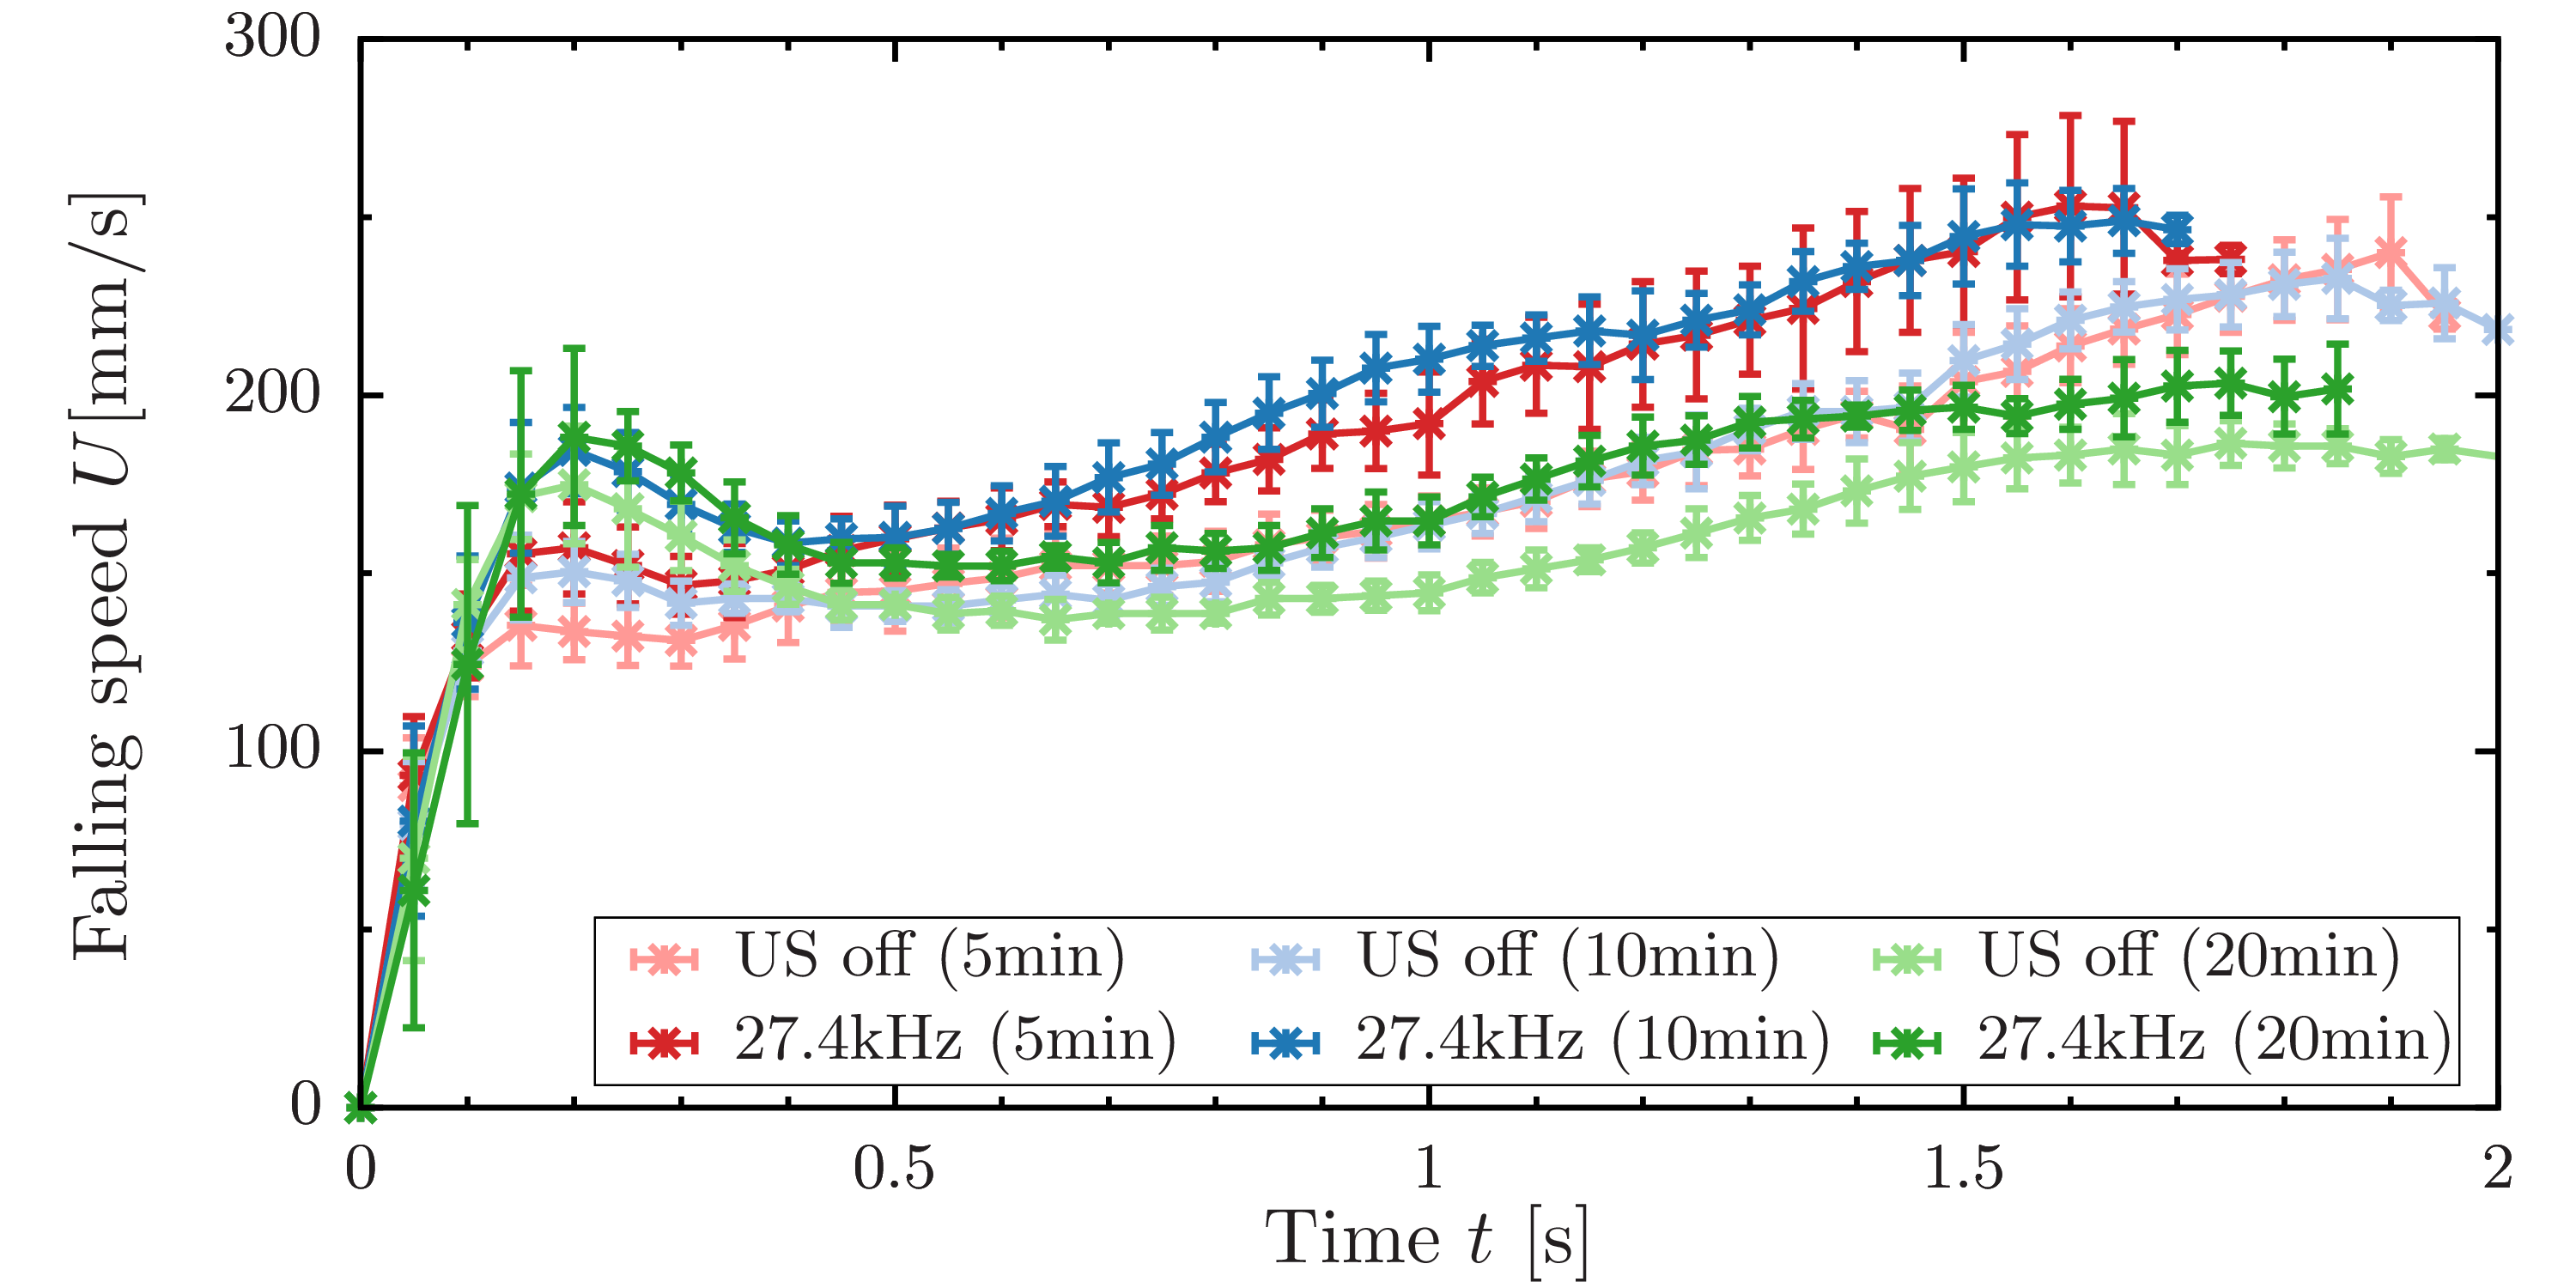
\includegraphics[width=13cm,clip]{5-Discussion/interval.png} 
        \caption{Drop interval change Experimental results.}
        \label{fig:interval-change}
    \end{center}
\end{figure}

\begin{figure}[ht]
    \begin{center}
        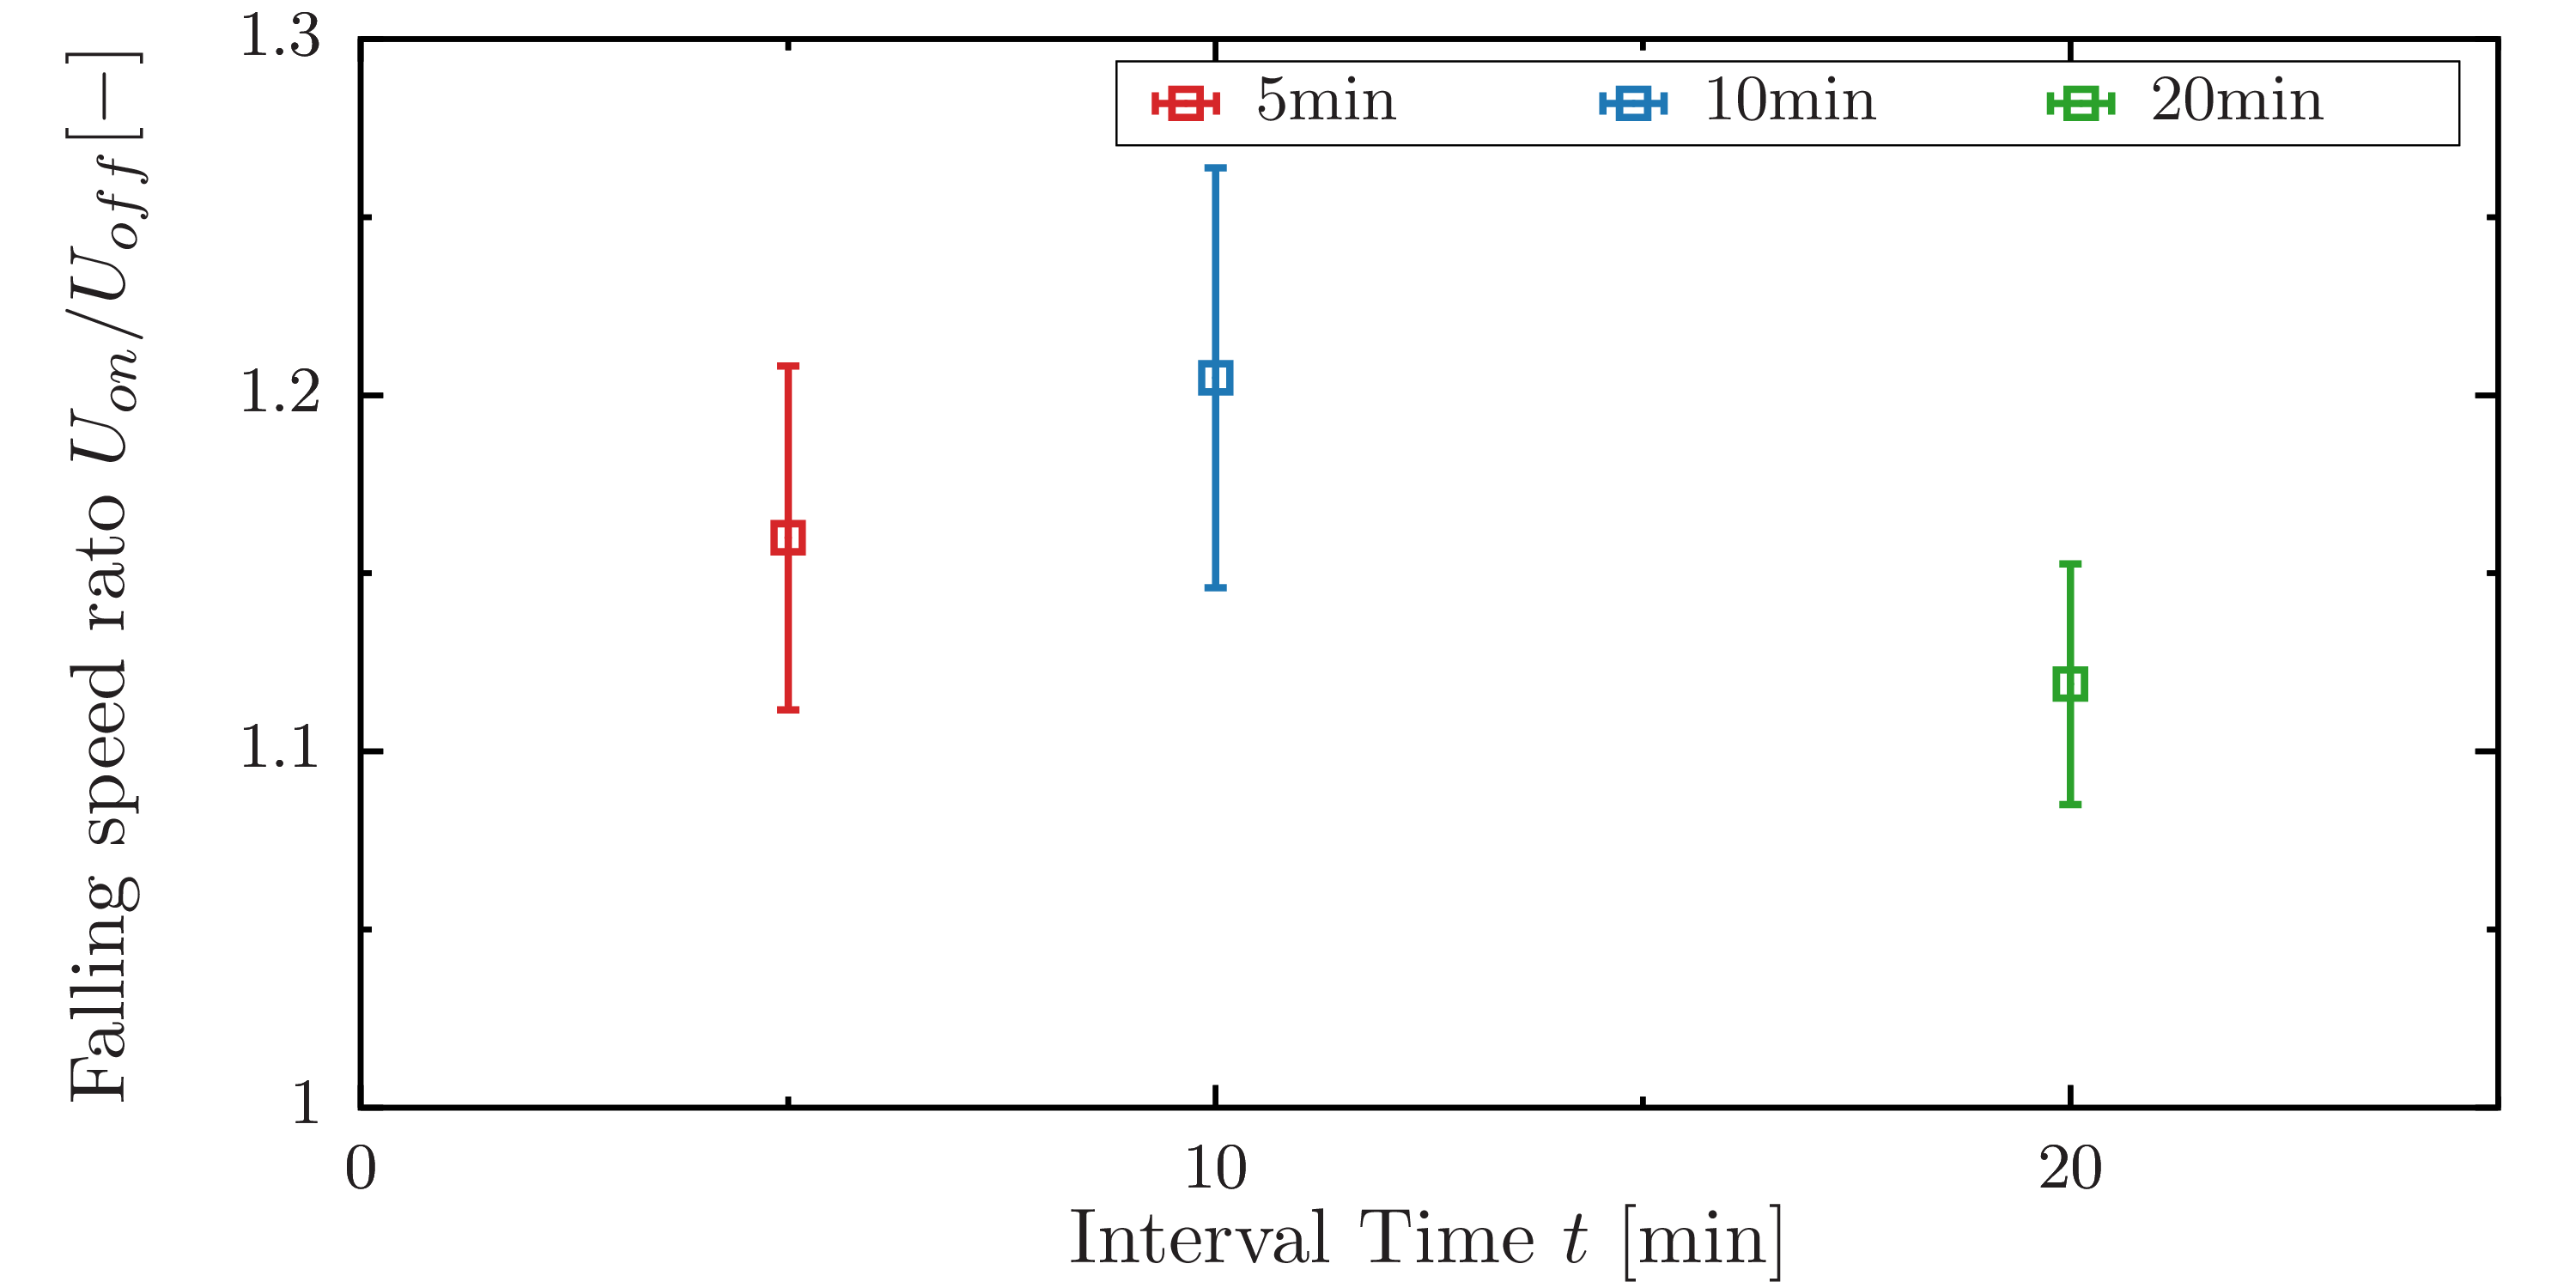
\includegraphics[width=13cm,clip]{5-Discussion/diff.png}
        \caption{Fall velocity ratio due to ultrasound irradiation with change in fall interval.}
        \label{fig:speed-diff}
    \end{center}
\end{figure}